% This is samplepaper.tex, a sample chapter demonstrating the
% LLNCS macro package for Springer Computer Science proceedings;
% Version 2.20 of 2017/10/04
%
\documentclass[runningheads]{llncs}
%
\usepackage{graphicx}
\usepackage{tabularx}
\usepackage{pgfplots}
\usepgfplotslibrary{external}
\usepackage{caption}
\pgfplotsset{width=\textwidth,compat=1.9}
% Used for displaying a sample figure. If possible, figure files should
% be included in EPS format.
%
% If you use the hyperref package, please uncomment the following line
% to display URLs in blue roman font according to Springer's eBook style:
% \renewcommand\UrlFont{\color{blue}\rmfamily}
\raggedbottom
\begin{document}
%
\title{Building a Knowledge Graph}
%
\titlerunning{BKG}
% If the paper title is too long for the running head, you can set
% an abbreviated paper title here
%
\renewcommand*\labelitemi{\textbullet}
\newcolumntype{Y}{>{\centering\arraybackslash}X}
\author{Lukas Bl{\"u}baum \and Nick D{\"u}sterhus \and Monika Werner}
%
\authorrunning{L. Bl{\"u}baum, Nick D{\"u}sterhus  et al.}
% First names are abbreviated in the running head.
% If there are more than two authors, 'et al.' is used.
%
\institute{University of Paderborn, Padeborn 33098, Germany \\
%\email{lncs@springer.com}\\ 
\email{\{lukasbl,nduester,mwerner\}@uni-paderborn.de} \\
\url{https://github.com/LukasBluebaum/BKG} 
% ABC Institute, Rupert-Karls-University Heidelberg, Heidelberg, Germany\\
%\email{\{abc,lncs\}@uni-heidelberg.de}
}
%
\maketitle              % typeset the header of the contribution
%
\begin{abstract}
The goal of this proseminar was to create an encyclopetic knowledge graph from a large text corpus like a wikipedia dump. In order to learn and better understand the basics of Semantic Web technologies. For this we were given a wikipedia dump and the core ontology of DBpedia. To facilitate this task we were introduced to several tools including FOX \cite{fox} and DBpedia Spotlight \cite{spotlight}. The whole project is written in Java and as license we used the GNU General Public License v3.0. The documented source code, including instructions on how to run the code, can be found on the given GitHub repository.

\keywords{Knowledge Graph  \and Semantic Web \and Coreference Resolution \and Named Entity Recognition
\and Entity Disambiguation \and Relation Extraction \and FOX \and Spotlight }
\end{abstract}


\section{Introduction}
Websites like Wikipedia contain a large volume of information. Unfortunately this information is mainly unstructured, for example in the form of natural language text. So the detection of complex informationen can be quite difficult. One approach to structure this knowledge is the extraction of triples from the natural language text. These triples consist of a subject, predicate and object and can then be displayed as a knowledge graph. The creation of such a knowledge graph is the main goal of this project. \\

To carry out this projekt several steps had to be taken. At first we had to process the given wikipedia dump and the core ontology. For the wikipedia dump this meant cleaning the text and for the core ontology we filtered some not required information. The next steps included Named Entity Recognition, Entity Disambiguation and Relation Extraction.
As frameworks for the Named Entity Recognition and Entity Disambiguation we used FOX and Spotlight. For the Relation extraction we implemented to approaches. The first approach takes the sentences and sends them to FOX in "re" mode to directly extract the triples. The second one, our own approach, uses Spotlight and the Stanford Core NLP \cite{stanford}. Finally we evaluated the results in relation to runtime and correctness. Here we measured how many triples from DBpedia we extracted per article, and manually checked the correctness of triples that are not contained in DBpedia. Due to time constraints we chose the category of U.S. Presidents for the evaluation.

\subsection{Architecture}
Just a few points to the architecture of our project. We used the WikiCleaner and OntologyParser classes to process the given DBpedia ontology and wikipedia dump. Then the RelationExtraction class starts two threads, one for the FOX approach and one for our own approach These two threads then try to extract the triples with the help of the NLPParser class and the webservices classes that query the online FOX demo and Spotlight demo respectively. As the last step the extracted triples will be written to a RDF graph.

\begin{figure}
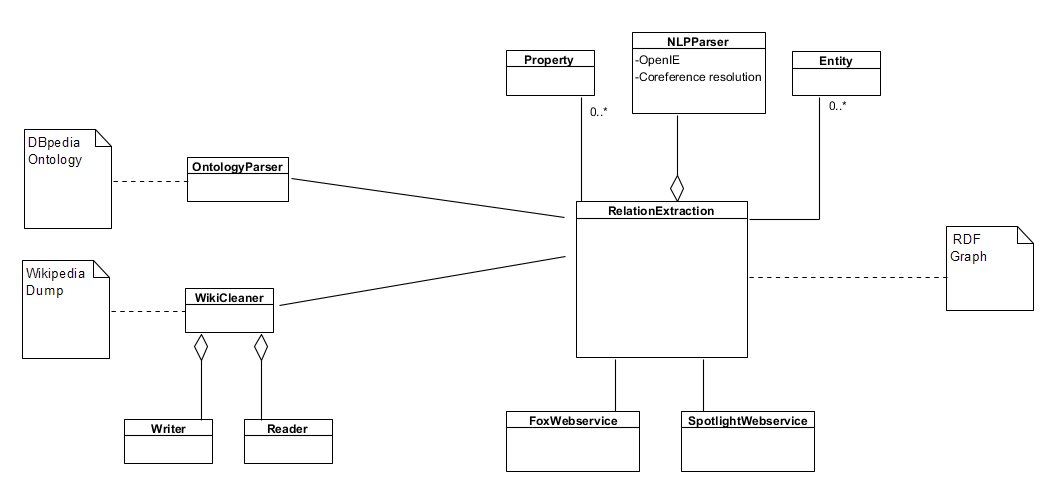
\includegraphics[width=\textwidth]{architecture.png}
\caption{A quick overview of the architecture of our project.} \label{fig1}
\end{figure}


\section{Preprocessing}
The preprocessing consists of the cleaning of the wikipedia dump and the coreference resolution.
\subsection{Extraction and cleaning of the text from a wikipedia dump}
As the foundation we were provided with a wikipedia dump. This wikipedia dump already came without markup, infoboxes 
or chapter subdivisions. The fact that there are no infoboxes already presented some problems, but more to that during the evaluation and discussion. But there were still some elements that were undesired for the later steps in this process. Such elements include unnecessary URLs, text in parenthesis, whitespace, nullchars and special symbols. We removed the texts passages in parenthesis because the Stanford CoreNLP had some problems with these during the binary relation extraction for our own approach later on. The elements were removed under application of some regular expressions. 
\pagebreak

The result is a simple text containing only the letters from the english alphabet, numbers, periods, commas and of course simple spaces. In order to speed up the cleaning process, we used a combination of Reader,Worker and Writer threads. To handle the concurreny we used BlockingQueues from the standard Java libraries. One which the Reader thread uses to pass the read lines to the Worker threads and another one which the Worker threads use to pass the cleaned lines to the Writer thread.


\subsection{Coreference Resolution}
Another step that needs to be taken before the information can be properly extracted is the coreference resolution, so that Spotlight and FOX can also recognize named entities in sentences were previously only a coreference appeared. Therefore we have to replace the pronouns with their representative mention. To actually find this representative mention we used the coref annotator \cite{coref} of the Stanford CoreNLP.  

\begin{example} John met Judy in 1960. He married her during his college year.\end{example}

In this sentence we obviously want to replace the he, her and his with their corresponding representative mention.
The result would look like this: 

\begin{example} John met Judy in 1960. John married Judy during John's college year. \end{example}


This example already shows one of the challenges that arise during the coreference resolution. Possesive pronouns have to be detected and handled accordingly. So in this case \textit{his} should not be replaced with \textit{John} but rather with \textit{John's}. To make this distinction we use the dependency parser \cite{parser} of the Stanford CoreNLP. Here we take the pronoun in question and then determine if it appears in connection with a possesion modifier relation. If it does, we adjust the representative mention the pronoun will be replaced with accordingly.



\section{Named Entity Recognition}
For this step we use the DBpedia Spotlight web service. We send the text to DBpedia Spotlight and receive a JSON response. The response is then parsed and the found entities and their information is stored in objects of our Entity class. As information we keep the uri, surface form, offset and the types. Since we send more than one sentence at a time to Spotlight we need to keep the offset to map the entities back to their corresponding sentence where they appeared. The surface form we need later on for our own relation extraction where we have to locate the entities inside binary relations. In addition to that we also keep the types because during our own relation extraction we compare these to the range and domain of some properties.





\section{Entity Disambiguation}
The Entity Disambiguation itself is already done by Spotlight and FOX. Spotlight for example has two approaches for this.
After they have located a candidate they take the information next to the surface form as information and try to determine the best match based on that. They also try to weigh words on their ability to actually disambiguate between candidates \cite{disambiguate}. FOX and AGDISTIS \cite{agdistis} \cite{agdistis2} were already discussed in the lecture.

\section{Relation Extraction}

\subsection{Using FOX}
FOX, can be used additionally to our relation extraction algorithm. FOX and our algorithm run in different threads in order to increase the number of triples with a reduced runtime. Here we just request FOX in 're' mode and then parse the output and write the triples that were found to the graph.
\subsection{Own Approach}
Our algorithm relies on the coreference resolution as well as Stanford OpenIE.
Third person pronouns are replaced by their representative mention. Our algorithm tries to send as many sentences as Spotlight can handle at once to reduce the number of requests which leads to a reduced runtime. Moreover, this provides Spotlight more context to perform disambiguation. \\

We build an entity class to save all the information we received, including the offset and the surface form to match the entities back to the sentences as well as the types. Those types are triples itself, but they are also needed to determine which properties would be a valid match according to their respective domain and range.
In the next step, we had to process Wikipedia sentences to extract binary relations between entities. Since Wikipedia sentences tend to be more complex simple dependency parsing can lead to failure.
We decided to use OpenIE, a system that extracts binary relation triples from a text. OpenIE recursively traverses the dependency tree to find independent clauses. It then searches for shorter arguments that are logically entailed by the original sentence. It also uses a proof system to only create logically coherent clauses.
We precompute the relations and save them for each sentence. \\

With the entities and relation stored the next task is to map those to DBpedia properties. Therefore we parse the DBpedia ontology and create Property (Relation) Objects. Each Property Object contains the label, domain, range and a number of keywords that allow us to map the property to natural language text. The first list of keywords is generated from the property labels. 
The properties are stored as a list, converted to JSON and saved as a file that we could manually or automatically edit.
A keyword String attribute that consists of multiple words, can be interpreted as a vector of which all words have to be found to map a relation to the property. We worked with lemmatized keywords and binary relations to reduce the needed amount of keywords. \\

We then iterate through all the entities and binary relation for a sentence and try to match the subject and the object of the binary relation to entities. Afterwards we map the keywords to the binary relation and check for the range and type. If everything matches we create a triple and write it to the graph. \\

For entity to literal relations, we first match the subject of the binary relation to an entity. Then we search for numbers inside the object. In case that we also find a month and two numbers we convert them to the xsd:date format. If we only find a number, we keep this number for the keyword matching step. Often Wikipedia plain text literals are partly written-out. To account for these cases we convert them to the actual number. 
\begin{example} 82 million $\Rightarrow$ 82000000 \end{example}
   
\section{Example}
In the following we will demonstrate the whole process at an example.

\begin{example}
Obama was born on August 4, 1961, at Kapiolani Medical Center for
Women and Children in Honolulu, Hawaii. He graduated from Harvard
University.\end{example}

After the coreference resolution the sentence will look like this: 

\begin{example}
	Obama was born on August 4, 1961, at Kapiolani Medical Center for
	Women and Children in Honolulu, Hawaii. Obama graduated from Harvard
	University.\end{example}

Next we use OpenIE to extract binary relations from the sentences, some of them are listed in the following table.


\begin{table}
		\caption{Shortened version of the binary relations extracted by OpenIE. (only some of the important ones we can actually use)}\label{tab1}
	\begin{center}
		\begin{tabularx}{\textwidth}{@{}|l|l|Y|@{}}
			\hline
			\textbf{Subject} &  \textbf{Predicate} & \textbf{Object}\\
			\hline
			Obama &  be bear on & August 4 1961\\
			Obama &  graduate from & Harvard University\\
			Obama &  be bear at & Kapiolani Medical Center for Women in Honolulu\\
			\hline
		\end{tabularx}
	\end{center}
\end{table}

Then Spotlight will find the following Named Entities.

\begin{example}
\textbf{Obama} was born on August 4, 1961, at \textbf{Kapiolani} Medical Center for
Women and Children in \textbf{Honolulu}, \textbf{Hawaii}. \textbf{Obama} graduated from
\textbf{Harvard University} .\end{example}

Now as already discussed we will try to map the subject, predicate and object to entities, properties and entities or literals. Here we distinguish between entity to literal relation and entity to entity relation.

\begin{table}
	\caption{Mappings entity to literal relation. For the first binary relation of Table 1.}\label{tab2}
	\begin{center}
		\begin{tabularx}{\textwidth}{@{}|l|l|Y|@{}}
			\hline
			\textbf{Part of binary relation} &  \textbf{Keywords} & \textbf{Mapping}\\
			\hline
			Subject &  Obama & dbr:Barack\_Obama\\
			Predicate &  bear & dbo:birthDate\\
			Object &  August 4 1961  & 1961-08-04\\
			\hline
		\end{tabularx}
	\end{center}
\end{table}



\begin{table}
	\caption{Mappings entity to entity relation. For the third binary relation of Table 1.}\label{tab3}
	\begin{center}
		\begin{tabularx}{\textwidth}{@{}|l|l|Y|@{}}
			\hline
			\textbf{Part of binary relation} &  \textbf{Keywords} & \textbf{Mapping}\\
			\hline
			Subject &  Obama & dbr:Barack\_Obama\\
			Predicate &  graduate & dbo:almaMater\\
			Object &  Harvard University  & dbr:Harvard\_University\\
			\hline
		\end{tabularx}
	\end{center}
\end{table}
So finally we get these two triples and write them to the graph. In this example we could also find the triple with the birth place of Honolulu. 

\section{Benchmark and Evaluation}
Note that for benchmarking and evaluation we only used our relation extraction approach.
\subsection{Runtime}
We measured the runtime of 100 articles in length of characters per time in minutes (see the graph below). We considered articles of different lengths to demonstrate how the runtime develops if the articles get longer. A huge share of the runtime is due to the coref annotator of the Stanford CoreNLP. This also explains the outliers because the coref Annotator then just takes longer for these sentences.

  


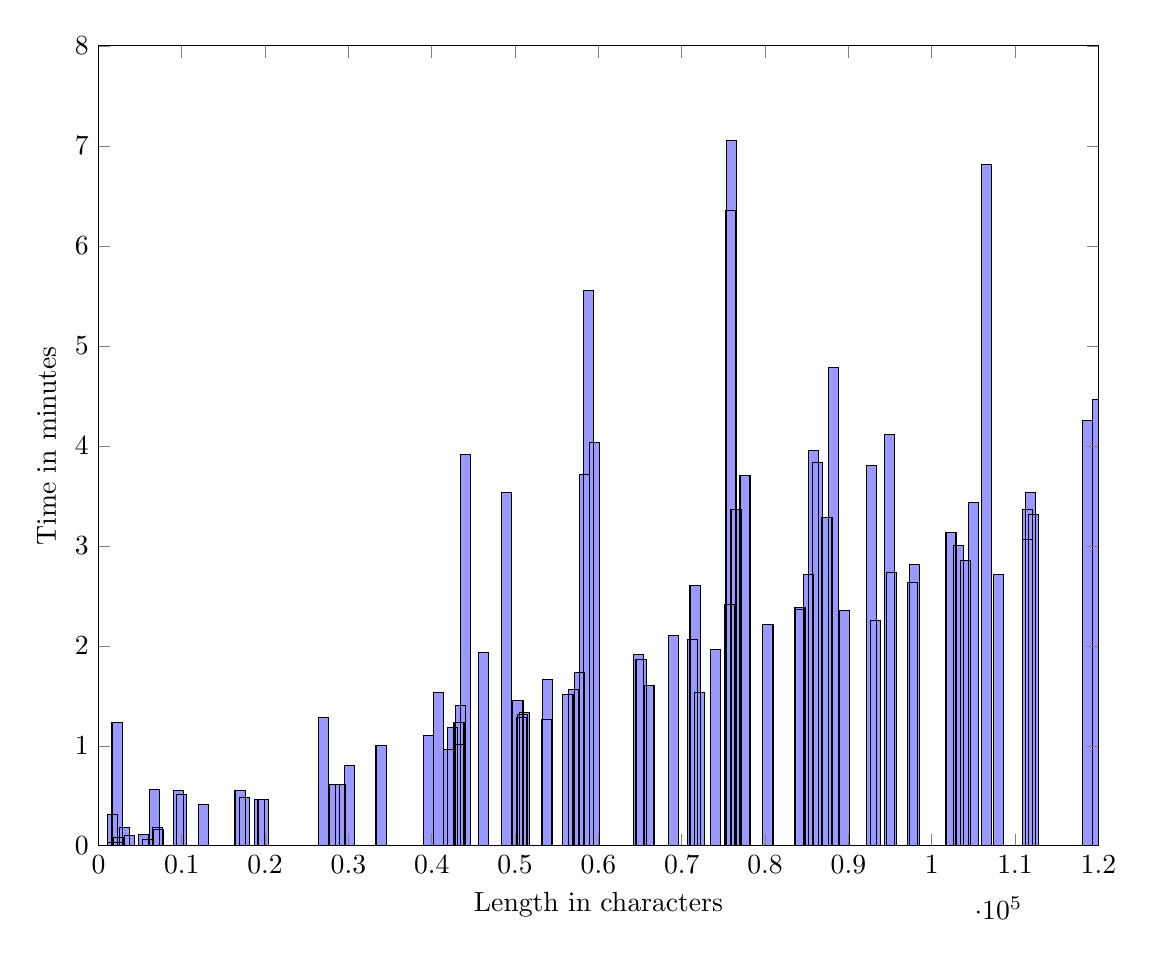
\begin{tikzpicture}

\begin{axis}[%
scale only axis,
width=5in,
height=4in,
xlabel=Length in characters,
ylabel= Time in minutes,
xmin=0, xmax=120000,
ymin=0, ymax=8,
axis on top]
\addplot[
ybar,
bar width=0.0502874in, 
bar shift=0in,
fill=blue!40,
draw=black] 
plot coordinates{ 
	(111453,3.3666666666666667) (94918,4.116666666666666) (85842,3.95) (85233,2.716666666666667) (50916,1.3166666666666667) (119839,4.466666666666667) (97655,2.6333333333333333) (95166,2.7333333333333334) (75964,7.05) (77587,3.7) (58296,3.716666666666667) (58807,5.55) (75869,6.35) (65114,1.8666666666666667) (87427,3.283333333333333) (57004,1.5666666666666667) (46195,1.9333333333333333) (104960,3.433333333333333) (89576,2.35) (102306,3.1333333333333333) (104061,2.85) (107992,2.716666666666667) (93254,2.25) (88178,4.783333333333333) (76518,3.3666666666666667) (118674,4.25) (48980,3.533333333333333) (74002,1.9666666666666666) (112234,3.316666666666667) (92795,3.8)
	(103164,3.0) (80339,2.216666666666667) (86315,3.8333333333333335) (111862,3.533333333333333) (56341,1.5166666666666666) (106587,6.816666666666666) (59495,4.033333333333333) (50342,1.45) (64839,1.9166666666666667) (53873,1.6666666666666667) (68984,2.1) (42456,1.1833333333333333) (71311,2.066666666666667) (97937,2.816666666666667) (3766,0.1) (9602,0.55) (53799,1.2666666666666666) (43464,1.4) (17488,0.48333333333333334) (12635,0.4166666666666667)  (84084,2.3666666666666667) (2444,0.08333333333333333) (2409,0.03333333333333333) (7190,0.16666666666666666) (33914,1.0) (43369,1.0166666666666666) (3174,0.18333333333333332) (75744,2.4166666666666665)
	(66070,1.6) (42017,0.9666666666666667) (5942,0.06666666666666667) (28364,0.6166666666666667) (9997,0.5166666666666667) (2238,1.2333333333333334) (5458,0.11666666666666667) (51101,1.3333333333333333) (1642,0.31666666666666665) (19755,0.4666666666666667) (29098,0.6166666666666667) (50725,1.2833333333333334) (16995,0.55) (19289,0.4666666666666667) (43271,1.2333333333333334) (7043,0.18333333333333332) (6724,0.5666666666666667) (44063,3.9166666666666665) (40813,1.5333333333333334) (111453,3.066666666666667) (72158,1.5333333333333334) (84186,2.3833333333333333) (27028,1.2833333333333334) (71598,2.6) (57741,1.7333333333333334) (39596,1.1) (30098,0.8) (1648,0.03333333333333333)
};

\end{axis}
\end{tikzpicture}
\subsubsection{Computer Specifications}
\begin{itemize} 
	\item OS: Windows 10 
	\item CPU: Intel Core i5-7600K 
	\item SSD
\end{itemize}
\subsection{Correctness}
For the evaluation we wrote a Benchmark class that takes a category and one or more dumps as input and then queries all subjects from the given category. Then we compare all triples from our graph that have a subject from the category with those from the dumps. \\

We selected the category \textit{Presidents of the United States}. First we compared our result to the given dumps, then we selected 100 triples randomly that were not contained in the dumps and checked them manually.\\

From the 2810 triples contained in the dump - from the chosen category - we also found 556. Note here that this also contains types we received from Spotlight, without the types these numbers are 2320 and 121. From the 100 randomly selected triples 46 were correct. This leads to a recall 
of 0.197 and precision of 0.46. So the resulting F-measure amounts 0.27. In the evaluation folder on the GitHub repository we provided the used files.
\subsubsection{The provided dumps (2016-10)} 
\begin{itemize} 
	\item disambiguations\_en.ttl, instance\_types\_en.ttl, labels\_en.ttl, long\_abstracts\_en.ttl,
	mappingbased\_literals\_en.ttl, mappingbased\_objects\_en.ttl, persondata\_en.ttl, specific\_mappingbased\_properties\_en.ttl, transitive\_redirects\_en.ttl
\end{itemize}


\section{Discussion}
In conclusion, our system can find relations from plain text utilizing two different strategies by FOX and our own algorithm. Our software relies on Spotlight for Named Entity Recognition and Stanford CoreNLP with OpenIE as our main tool to extract logically coherent relations.
By coreferencing the articles we can consider each sentence for itself. Our algorithm scales with the amount of keywords that are added to the mentioned property file. It can theoretically find relations for all DBpedia properties, besides Entity to String relations since we lack context to reach a good precision on those. \\ 

In the following we will discuss some difficulties and possible improvements. Many triples can only be found in the infoboxes so we cannot find them in the text itself. For example the height of a person. We only focused DBpedia ontology properties - except types and names - so it can distort the benchmarking since our system is not designed to find properties based on the structure of the text like dbo:abstract or other namespaces like $<$http://purl.org/dc/terms/description$>$. We also missed some triples or extracted incorrect ones because of the disambiguations. For example Spotlight often falsely recognized parties not as the actual party but rather as the history of that party. In addition to that the disambiguation also fluctuated depending on the amount of text.\\

The main improvement that could be made, would be to adjust the information including the keywords for the properties. Since sometimes we miss context if the property lacks the domain and/or range. For example dbo:citizenship not having range dbo:Country. A huge number of carefully selected keywords or maybe even negative keywords so words that should not occur would also improve the property selection. 

 
% ---- Bibliography ----
%
% BibTeX users should specify bibliography style 'splncs04'.
% References will then be sorted and formatted in the correct style.
%

\bibliography{references}
\bibliographystyle{splncs04}
%


\end{document}
